% !TEX root = ../PhD Thesis.tex
\chapter{CompBio app server}
\label{chap:app-server}

Since I started building psichomics, I wanted my work to be publicly available as an online web app, providing users the most up-to-date version at their fingerprints, without having to install, update and manage different versions of R, Bioconductor, psichomics and all their dependencies.
%It can take an hour to install psichomics from scratch and the command line may scare the end-users for whom psichomics was created. 
Five years after the first Bioconductor release of psichomics in 2016, that vision finally came true.

\begin{figure}[!b]
  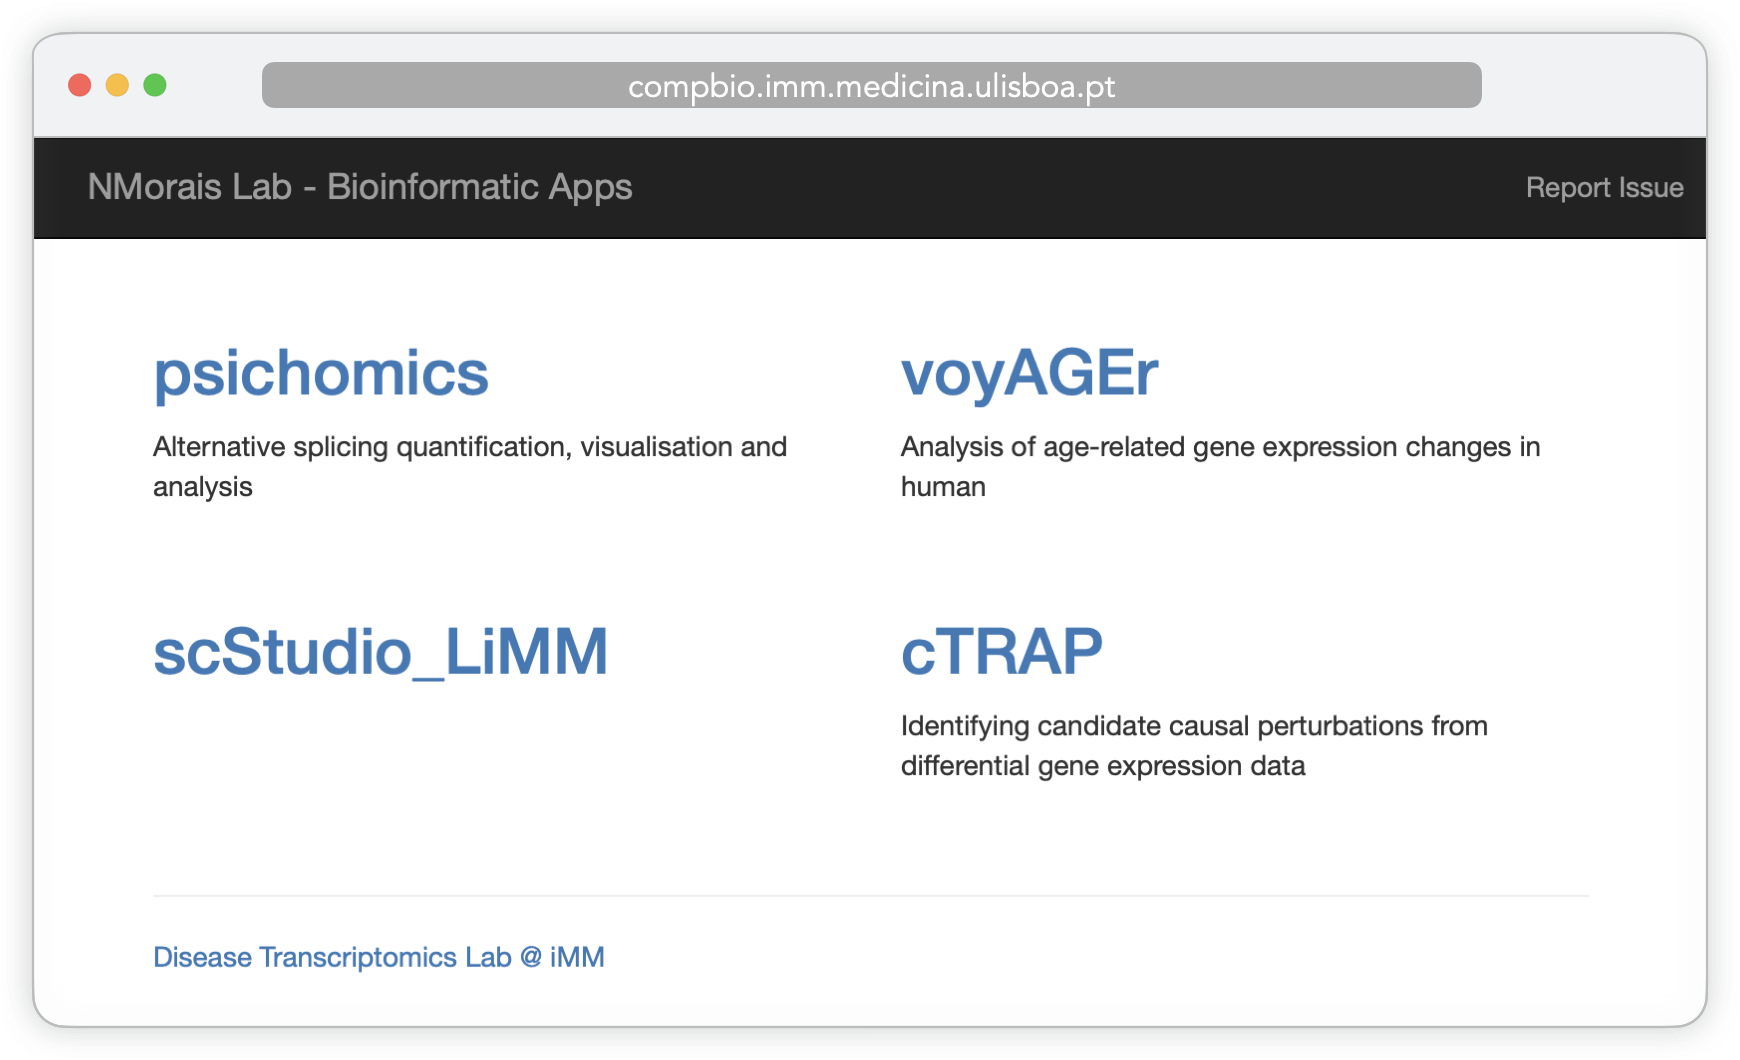
\includegraphics[width=.89\textwidth]{images/app-server/homepage}
  \centering
  \caption[Screenshot of CompBio's homepage]{\textbf{CompBio's homepage screenshot.} List of hosted web apps (11 Nov 2021).}
  \label{fig:homepage}
\end{figure}

One of our lab's ambitious goals is to develop interactive visual tools to assist in exploring biological data, either provided by users or available from big datasets. These tools need to be easily reachable to be used by everyone, no matter their computational background. To turn that dream into reality, I set up the CompBio app server, a Linux virtual machine running in iMM computing cluster that hosts psichomics, cTRAP and other Shiny apps from my lab colleagues. The server is accessible at \alink{compbio.imm.medicina.ulisboa.pt} (\autoref{fig:homepage}) and its code at \alink{github.com/nuno-agostinho/compbio-app-server}.

% TODO: write specs of the app server? 200GB SSD, 64GB RAM, 16 CPU threads

\section{Background}

Our lab uses the R programming language to analyse clinical and molecular data from public sources or collaborators. An R package that we have been using more and more in the lab is Shiny (\alink{shiny.rstudio.com}) that allows to build interactive web apps, particularly useful to create exploratory dashboards to be shared with our collaborators or even the whole scientific community. When starting to create Shiny apps, it is natural to wonder: what is the best way to share them?

\subsection{Desktop apps}

Shiny apps are written in R, an interpreted programming language that allows to run the source code in multiple platforms. When run locally, the Shiny app starts running in the device itself (\texttt{localhost}) and that can be open by any web browser. Shiny apps can be provided just like any other R package in CRAN or Bioconductor (such as in the case of psichomics and cTRAP). However, this requires the user to install multiple programs in their computer: R, Shiny, the Shiny app, and all their dependencies. Therefore, Shiny apps by themselves are not sufficient to make it easier to access apps because of all the dependencies that are required to install\footnote{Installing psichomics in a new system with R installed can take up to 1 hour.}.

% Java (\alink{java.com}) is a platform-independent, general-purpose programming language intended to allow the same code to target multiple platforms. It uses an intermediary Java virtual machine (JVM) that translates Jave bytecode to the native platform's language. On the other hand, graphical interfaces in Java can consume more time and memory than native apps, besides having a user interface that is in stark contrast to the graphical interface of other apps.

One way to reduce the number of dependencies when locally installing a Shiny app is to use Docker (\alink{docker.com}), allowing to run isolated Linux virtual environments (containers) with programs and all their dependencies. A problem with this approach is that end-users are required to install Docker to run Docker containers, a program that requires admin privileges that (1) not all users may have and (2) they may not feel comfortable to give those privileges.

A replacement is Electron (\alink{electronjs.org}), a software framework that allows to develop cross-platform graphical user interface apps using web technologies by combining a web browser rendering engine (Chromium, used in Chrome and other web browsers to convert HTML and CSS code into an interactive web page) and a JavaScript environment (node.js). The app itself would run the web app as if it were a usual desktop app. Some open-source projects like electricShine (\alink{github.com/chasemc/electricShine}) and photon (\alink{github.com/COVAIL/photon}) allow to convert Shiny apps to Electron apps. However, compared to native apps, Electron apps are slower, have a significant overhead, take more space and consume more RAM, making Electron less attractive for intensive data-processing apps.

\subsection{Web apps}

In contrast to native desktop apps, web apps are cross-platform and always up-to-date. However, they require computing resources from a web server that is constantly online and that may balance the resources across multiple users. The required resources to allocate to a web server depend mainly on the amount of RAM, storage and CPU threads desired according to resources consumed per app, the number of active users at the same time and the data storage.

Multiple web app hosting services support Shiny apps, including Heroku (\alink{heroku.com}) via Docker containers and \alink{shinyapps.io}. Both of these app hosting services offer subscription plans depending on allocated system resources, including a free plan useful to run basic Shiny apps: Heroku's free plan offers 2 threads, 512 MB of RAM and 500 MB of storage per app\footnote{According to Heroku (\alink{heroku.com/pricing} and \alink{devcenter.heroku.com/articles/limits}) as of 24 November 2021. Unverified accounts (i.e. not associated with a valid credit card) are limited to 5 apps.}, whereas \alink{shinyapps.io}'s free plan allows for 5 active apps with 25 computing hours per month using 1024 MB of RAM and 1 GB of storage per app\footnote{According to official \alink{shinyapps.io} documentation (\alink{docs.rstudio.com/shinyapps.io/applications.html} and \alink{shinyapps.io\#pricing}) as of 24 November 2021.}. Such services take care of deploying the web apps and we can easily pay to scale the required resources to run the apps, according to their usage. They also allow to easily monitor app resource usage to understand how the apps are being used and if the resources employed are sufficient or not without much effort to the developer.

Instead of using third-party app hosting servers, Shiny apps can be deployed in local web servers. This requires server maintenance and may be harder to scale resources. The following programs allow to host Shiny apps in a local machine:

\begin{itemize}
	\item \textbf{Shiny Server} (\alink{rstudio.com/products/shiny/shiny-server}) is a bare-featured open-source program with only the essential features to host Shiny apps.
	\item \textbf{RStudio Connect} (\alink{rstudio.com/products/connect}) is a paid program\footnote{According to RStudio (\alink{rstudio.com/pricing}), all RStudio commercial products are free for teaching purposes and 50\% discounted for academic research from their regular bundle pricing starting at 22000\$ per year as of 24 November 2021.} with many more features than Shiny Server, including user authentication, Python-based app support and resource usage metrics.
	\item \textbf{ShinyProxy} (\alink{shinyproxy.io}) is an open-source program to host Shiny apps in Docker containers with many of the features found in RStudio Connect, including user authentication, Python-based app support and resource usage metrics.
\end{itemize}

As we have sufficient computing resources, we decided to build an app server. Among the available programs to host Shiny apps with own resources, ShinyProxy has many of the advantages of using the proprietary RStudio Connect for free, so we went with ShinyProxy to host our Shiny apps. After selecting the main technology, we had to think how to properly develop the app server so it is easy to test, maintain and update.

% Nginx as reverse proxy to handle all requests, including SSL certificates for HTTPS

\subsection{Building an app server}

There are a lot of programs that can go into a web server. Experimenting different programs while managing their manifold dependencies to develop an healthy web server is like an intricate ballet where all finely-coordinated dancers interplay for an astounding performance. This can be as difficult as it sounds: a wrong move can affect the whole show. After all, each program/dependency has its own requirements and some may be a distress to (un)install. Moreover, when the server is online, errors may arise due to configuration changes (such as new app updates), requiring a fast rollback to minimise server downtime. A solution is to use self-contained and modular programs, such as in the case of Docker containers. But how to coordinate several Docker containers to beautifully perform the Swan Lake?

With Docker Compose, a program to manage multiple Docker containers simultaneously, multiple applications are run isolated from others in their own Docker containers, allowing to easily update or replace them without affecting other system components. All services spawned in Docker Compose are Docker images, either pre-created (e.g.  Docker images from Docker Hub) or built before starting up all services (in this case, a Dockerfile is required to create the Docker images). Docker Compose allows to quickly play and swap programs: the services present in the server were selected after trying out many other combinations of alternative apps. The modularity of Docker Compose allows to easily test new system components and update software versions.

Nginx as a reverse proxy, serves as an intermediary between the user requests and the server.

In this chapter we describe CompBio, an app server built with Docker Compose and multiple interacting services to allow for R/Shiny and Python app deployment (ShinyProxy), reverse proxy (Nginx), background tasks (Celery, Redis and Flower), website analytics (Plausible, PostgreSQL and ClickHouse), resource monitoring (Prometheus and Graphana), and development purposes (RStudio Web, not used in production).

CompBio is currently running in a virtual machine in a Linux computing cluster and hosts Shiny apps from NMorais lab, including the tools previously mentioned in this document, psichomics and cTRAP. CompBio is freely available at \alink{compbio.imm.medicina.ulisboa.pt}.

\section{Materials and methods}

CompBio is built using Docker Compose and includes the Docker images of multiple services: ShinyProxy, Nginx, Celery, Redis, Flower, Plausible, PostgreSQL, ClickHouse, Prometheus, Grafana and RStudio Web (\autoref{tab:compbio-services}). 
RStudio Web is only available in the development profile. The services communicate between each other via a single network created by Docker (\autoref{fig:architecture}).

\begin{table}
\small
\caption{\textbf{CompBio services.}}
\label{tab:compbio-services}
\begin{tabularx}{\textwidth}{ l l l }
\toprule
\parnoteclear
\textbf{Role}                    & \textbf{Service} & \textbf{Docker image}\parnote[a]{Available in Docker Hub, unless stated otherwise.} \\ \toprule
Web app deployment                   & ShinyProxy       & \dockerlink{openanalytics/shinyproxy}     \\ \midrule
Reverse proxy                        & Nginx            & \dockerlink[_]{nginx}     \\ \midrule
\multirow{3}{55mm}{Background tasks} & Celery + cTRAP   & Based on \dockerlink{nunoagostinho/ctrap}\parnote[b]{Python and Celery are installed on top of cTRAP Docker image, allowing Celery to run cTRAP analyses: see file \link{https://github.com/nuno-agostinho/compbio-app-server/blob/main/celery/Dockerfile}{celery/Dockerfile}.} \\
                                     & Redis            & \dockerlink[_]{redis}     \\
                                     & Flower           & \dockerlink{mher/flower}     \\ \midrule
\multirow{3}{55mm}{Website analytics
\par(i.e. track visitor metrics)}    & Plausible        & \dockerlink{plausible/analytics}     \\
                                     & PostgreSQL       & \dockerlink[_]{postgres}     \\
                                     & ClickHouse       & \dockerlink{yandex/clickhouse-server}     \\ \midrule
\multirow{2}{55mm}{Register and monitor
\par server resources}               & Prometheus       & \dockerlink{prom/prometheus}     \\
                                     & Grafana          & \dockerlink{grafana/grafana}     \\ \midrule
Run R sessions and test features     & RStudio Web\parnote[c]{Only available in the development profile.} & Based on \dockerlink{rocker/rstudio} \\
\bottomrule
\end{tabularx}
\parnotes
\end{table}

\begin{figure}[!t]
  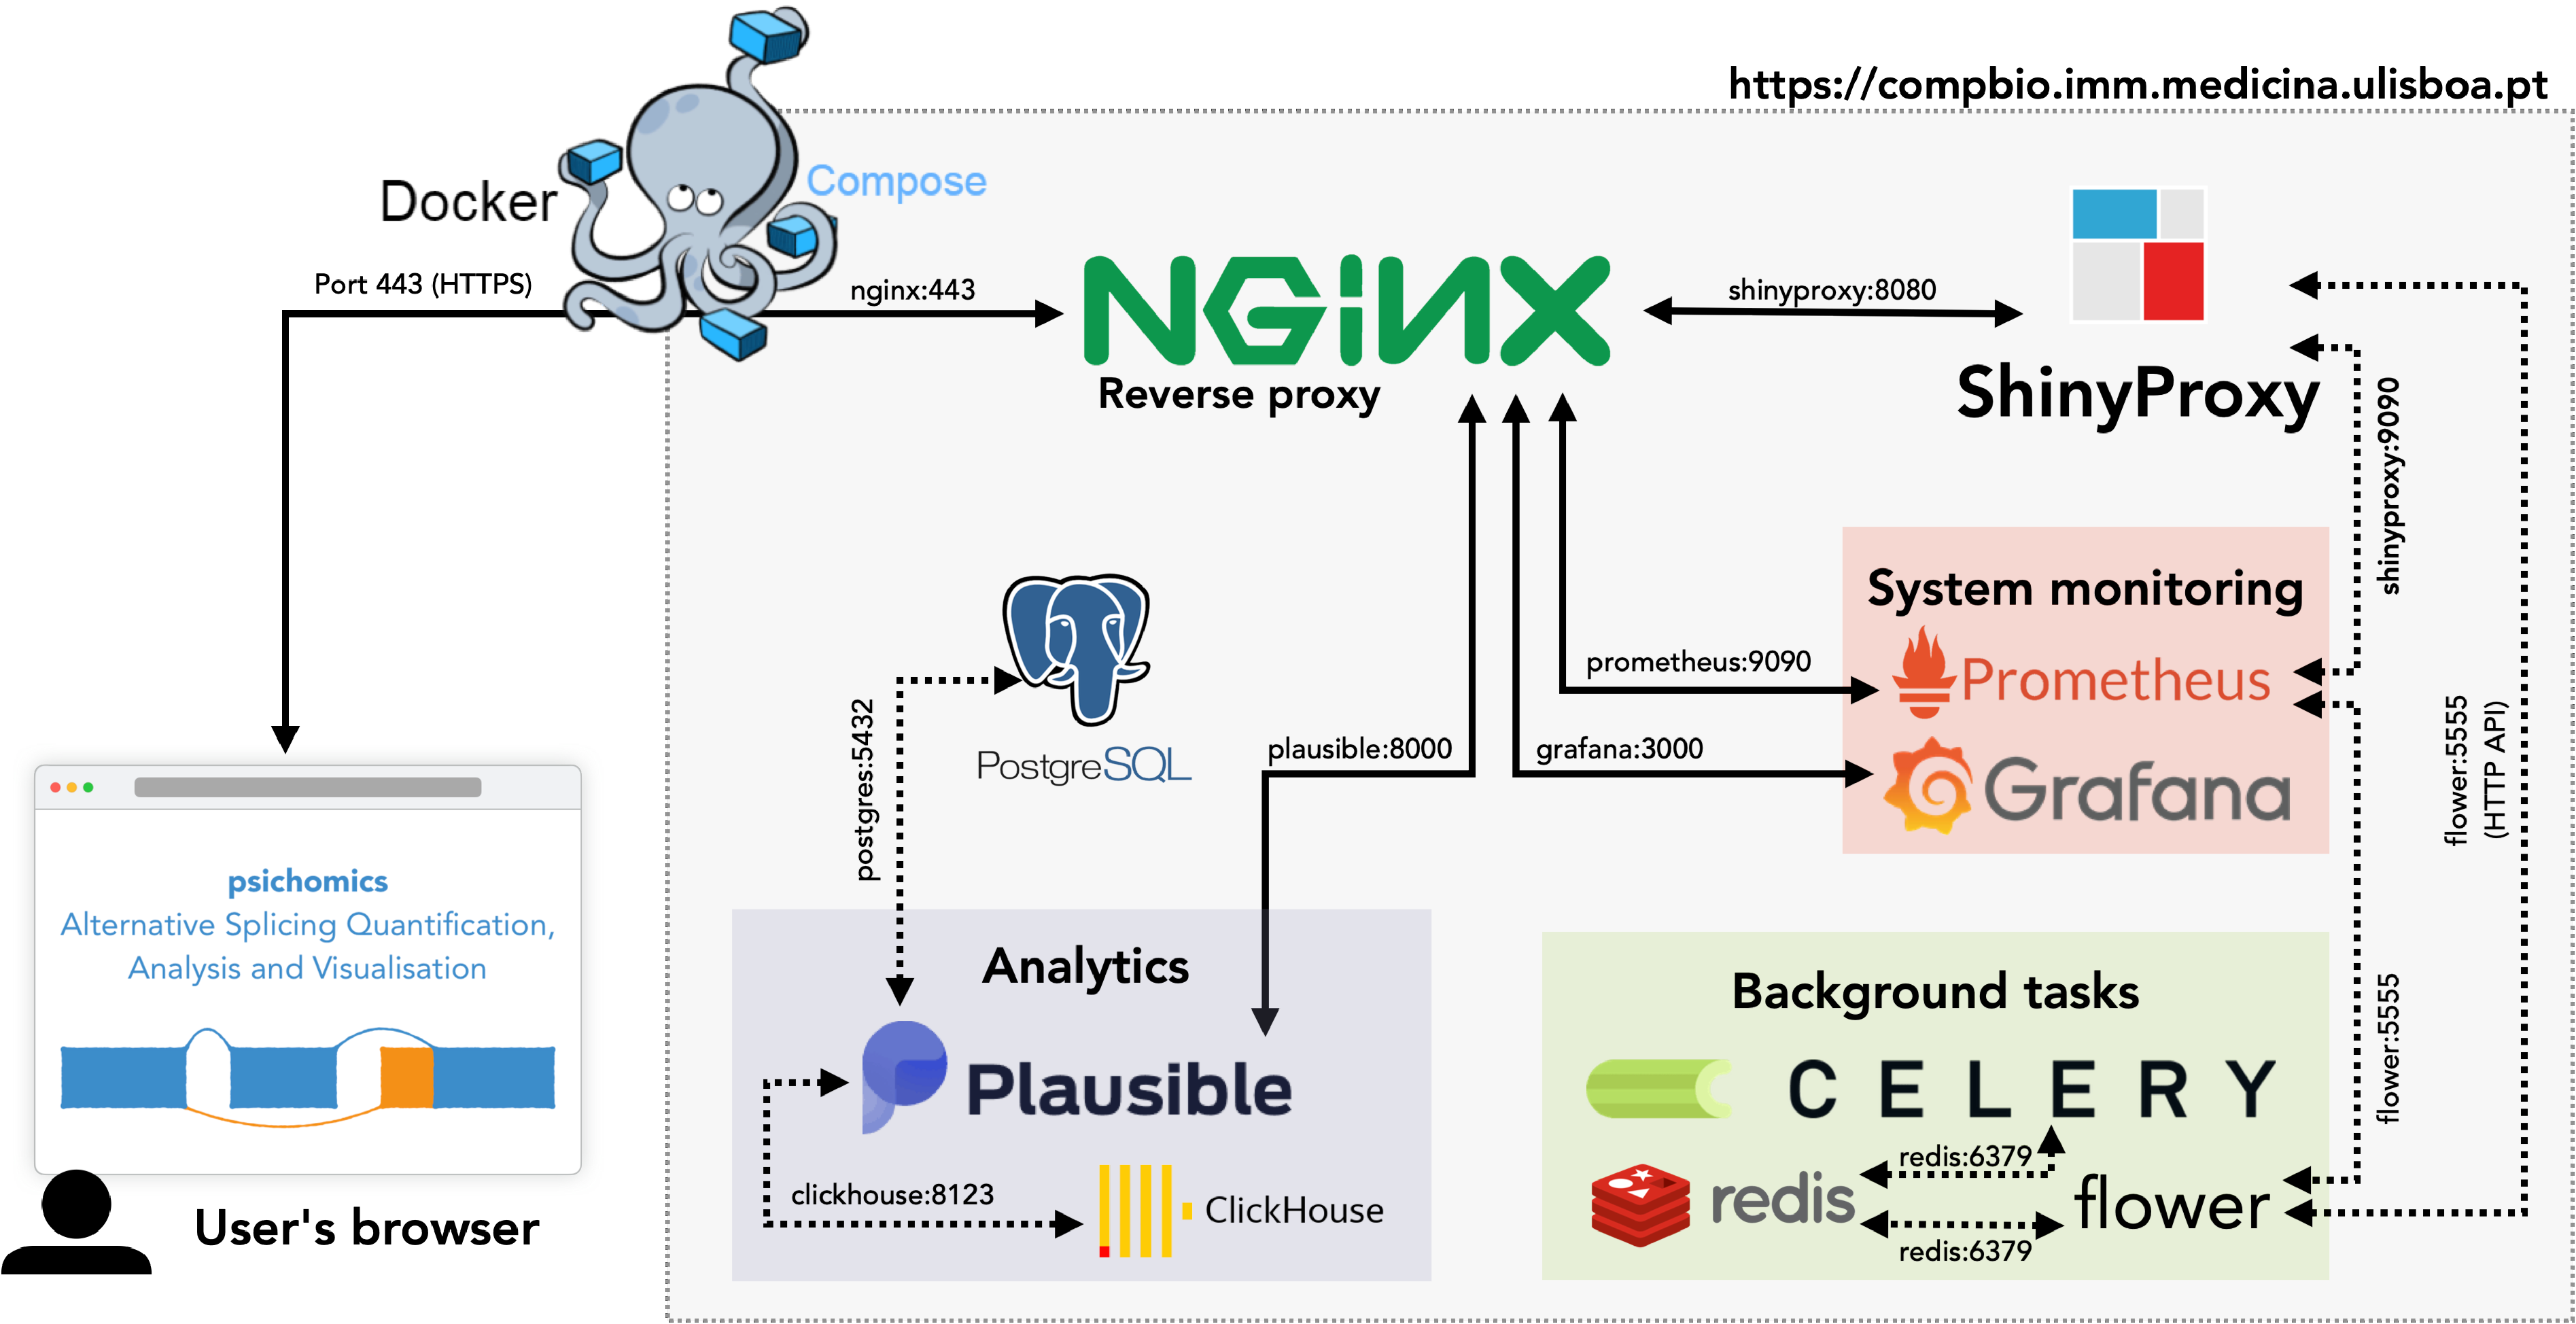
\includegraphics[width=.9\textwidth]{images/app-server/architecture}
  \centering
  \caption[App server architecture]{\textbf{App server architecture is based on Docker Compose.} All services are provided via Docker images and communicate with each other via a Docker-created network using the name of the service and a specific port (e.g. Nginx communicates with ShinyProxy via \texttt{shinyproxy:8080}). The groups  (analytics, system monitoring and background tasks) are strictly conceptual.}
  \label{fig:architecture}
\end{figure}

\section{Results}

The CompBio app server runs in Linux\footnote{CompBio may run in other operating systems. However, this is beyond the scope of this project.} machines with only Docker and Docker Compose as requirements, thus making the setup easily portable across different Linux computers and requiring minimal user setup.

\subsection{Docker Compose}

All the code required to run the app server is available at \alink{github.com/nuno-agostinho/compbio-app-server}. A single file (\texttt{docker-compose.yml}) contains the main configuration of each application in the server, and extra configuration files are available in the local directory. For organisation purposes, the project is organised by folders named after each service, where each folder stores files (e.g. Dockerfile, configuration and data) associated with the respective application (\autoref{fig:file-structure}).

\begin{figure}[!h]
  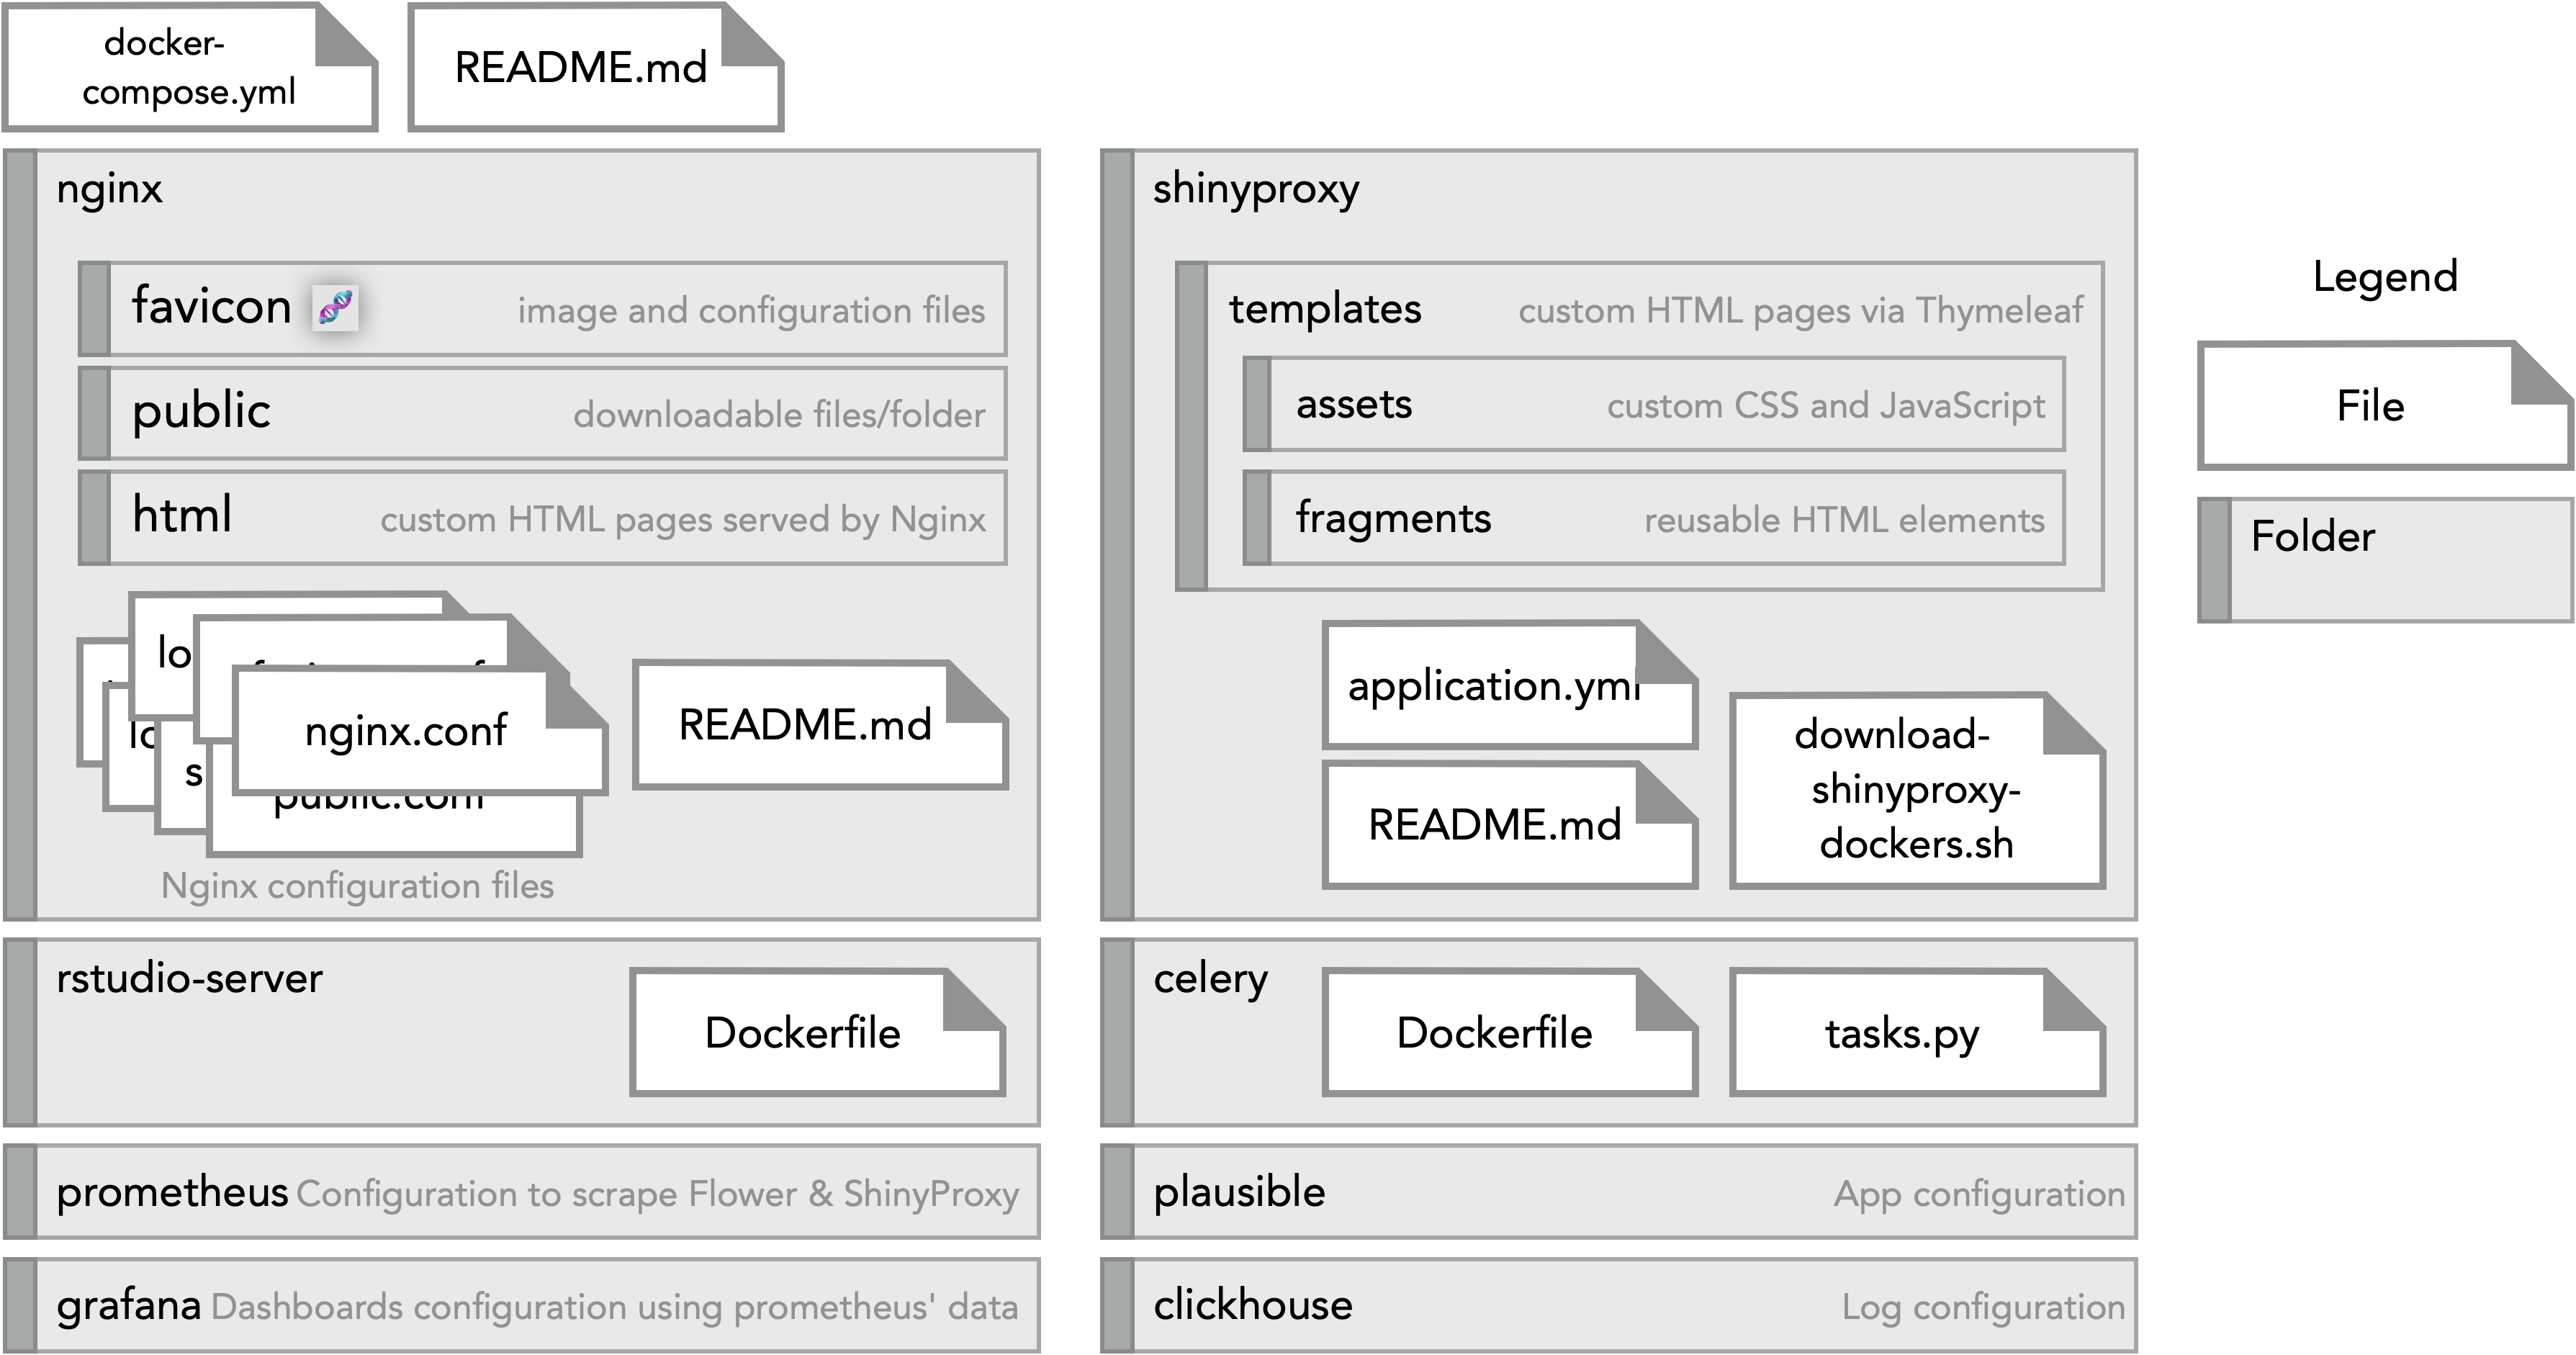
\includegraphics[width=1\textwidth]{images/app-server/file-structure}
  \centering
  \caption[App server's file structure]{\textbf{Visual representation of the file structure of the CompBio app server.} Each folder contains files associated with a specific service. Folders \texttt{rstudio-server} and \texttt{celery} contain Dockerfiles for building custom Docker images of the respective services.}
  \label{fig:file-structure}
\end{figure}

Although data from Docker containers are only available temporary after the container is stopped, important files are preserved in Docker volumes to avoid data loss when restarting services. Docker volumes are mounted when starting the \texttt{docker-compose.yml} project. Although data from Docker is temporary, specific directories are mounted in Docker volumes to be stored in the long-term (such as databases).

A single command is enough to build Docker images from Dockerfiles, download Docker images from Docker Hub and start up every service in detached mode\footnote{\texttt{docker-compose up -d --build}}.

Multiple \texttt{docker-compose} commands allow to manage the services. For instance, it is possible to restart single services without affecting other programs. This is specially useful when altering the configuration of a service. However, changes to \texttt{docker-compose.yml} are only applied after restarting all services by shutting down all services with \texttt{docker-compose down}.

% kubernetes?
% Ansible?

\subsection{ShinyProxy}

ShinyProxy is an open-source program that deploys R/Shiny and Python apps via Docker. When a user starts an app, ShinyProxy creates a new Docker container exclusively for that user. The containers are automatically terminated 30 minutes (by default) after the last user interaction.

Adding new apps to the system is as simple as pulling the Docker image of the app in the server and adding them to the ShinyProxy configuration file.

% ShinyProxy vs shinyapps.io vs other alternatives

ShinyProxy offers multiple built-in features, including:

\begin{itemize}
	\item \textbf{Usage statistics:} many ShinyProxy metrics (including app usage time, app failures and user numbers) are collected with Prometheus and visualised using Grafana.
    \item \textbf{App recovery:} when restarting ShinyProxy, ShinyProxy-initiated Docker containers continue running in the background and are attached once ShinyProxy finishes loading, minimising issues related with server maintenance. The apps will be unavailable while ShinyProxy is not running. For more information, please read \alink{shinyproxy.io/documentation/app-recovery}.
    \item \textbf{User authentication:} authentication with multiple methods, including social login via GitHub, LinkedIn, Google, etc. However, user authentication requires all visitors to login before continuing. As we prefer users to be able to anonymously access our apps, this feature is currently disabled.
    \item \textbf{User sessions:} user data can be stored in user-specific folders. As the sessions are only accessible when the Docker container is already attached to the volumes, this allows for complete isolation from other user folders. However, this feature works best with user authentication enabled (otherwise, random identifiers are used for each visitor and requires custom logic to load data between computers).
	\item \textbf{Multiple app instances:} users can open and manage multiple app instances simultaneously (not currently enabled in the app server); for more information, please visit \alink{shinyproxy.io/documentation/ui/\#using-multiple-instances-of-an-app}.
\end{itemize}

\subsubsection{Progress bar when loading ShinyProxy apps}

\begin{wrapfigure}{r}{.5\textwidth}
  \vspace{-\intextsep}
  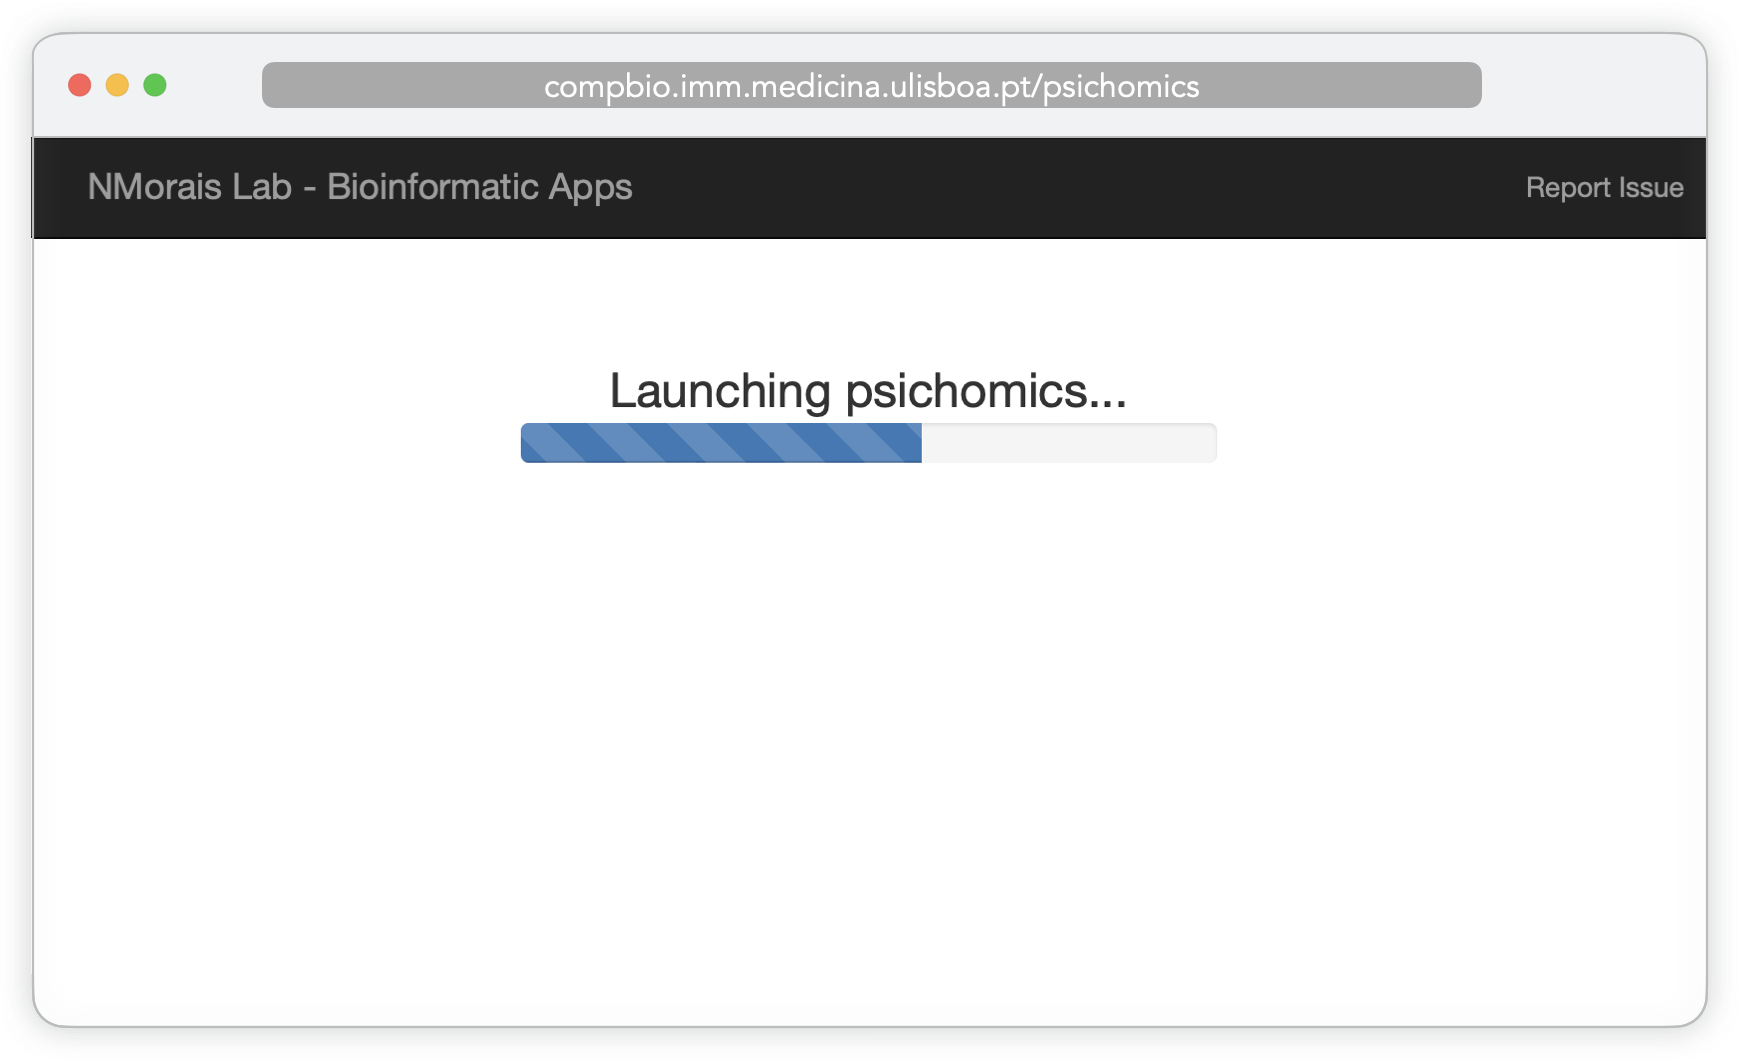
\includegraphics[width=\linewidth]{images/app-server/progress-bar}
  \caption[Screenshot of app loading]{\textbf{Progress bar displayed while psichomics loads} (11 Nov 2021).}
  \label{fig:progress-bar}
  \vspace{-\intextsep}
\end{wrapfigure}

% https://dl.acm.org/doi/pdf/10.1145/1294211.1294231
% https://www.chrisharrison.net/index.php/Research/ProgressBars2
% https://dl.acm.org/doi/pdf/10.1145/2702123.2702139
% https://www.researchgate.net/publication/234791131_The_importance_of_percent-done_progress_indicators_for_computer-human_interfaces
% https://ieeexplore.ieee.org/stamp/stamp.jsp?tp=&arnumber=6263888&tag=1

When ShinyProxy is loading an app, a spinning wheel is usually shown as a loading indicator. For apps that take more than 10 seconds to load (e.g. psichomics and cTRAP), this may give the feeling that the website is not working, as the perceived time taken to load is larger than elapsed time. %citation needed
To avoid that, the spinning wheel was replaced with a progress bar that provides users with a time estimate for app loading (\autoref{fig:progress-bar}). The progress bar fills based on time alone.

By default, the progress bar takes 5 seconds to fill (as sample Shiny apps take that much to launch in ShinyProxy), but the time is customisable for specific apps by editing a specific app in \texttt{shinyproxy/application.yml} and adding a \texttt{template-properties.start-up} parameter. For instance, psichomics takes 20 seconds to fully load the progress bar (i.e. \texttt{template-properties.start-up: 20s}), whereas cTRAP takes 15 seconds. When the app is loaded (regardless of the progress shown), the progress bar fades out.

%To create this progress bar, \verb|shinyproxy/templates/app.html| was edited to remove the spinning wheel and to include an empty progress bar. The progress bar's width is changed from 0\% to 100\% using JavaScript. By default, the CSS width transition applied to the progress bar is \texttt{transition: width 5s ease-in-out;} (animating a change of width that last for 5 seconds in an ease-in animation) where \texttt{5s} is replaced by the \texttt{template-properties.startup-time} parameter if set.

\subsubsection{Custom HTML pages}

\subsection{Nginx}

Nginx is a reverse proxy, i.e. an intermediary that decides what is shown to the user depending on the URL visited (akin to those switchboard operators seen in the old movies). In CompBio, Nginx is responsible to fulfil user requests, to ensure HTTPS traffic is encrypted via SSL certificates, serve publicly available files and show a custom error page if ShinyProxy is not responding (e.g. temporarily down or overloaded).

Nginx is also used for ensuring encrypted HTTPS traffic via SSL certificates. SSL certificates are handed by the IT team at iMM and we only need to point Nginx to the correct location of those certificates. SSL certificates include three separate parts: the site certificate, intermediate certificates, and the private key.

% public
A public folder is available via Nginx.

% custom HTML error page
In case ShinyProxy is down, Nginx will serve a custom error page stating that the server is down probably because of ShinyProxy. This is informative enough to end-users that know they should wait to refresh the page in a moment and also to admins that will understand that ShinyProxy is temporarily down (this can happen because of multiple reasons, such as a restart of the service or overloading).

% favicon

% An issue with Nginx is that it is especially verbose compared to more recent reverse proxies. I would have prefer to replace Nginx with a simpler reverse proxy such as Caddy (\alink{caddyserver.com}).

\subsection{Background tasks}
% Redis as database

% R is a single-process task
% Long-running tasks

% Celery is a Python app
% How does it run R?

\subsection{Website analytics}

Plausible is an open-source, privacy-focused web analytics tool that collects traffic metrics for multiple websites and provides them via an interactive dashboard. CompBio runs the self-hosted version of Plausible. All of Plausible metrics (e.g., visitor numbers, total page views and session duration) are anonymously aggregated without cookies, thus avoiding individual tracing.

% plausible + clickhouse + postgres
% postgres can be used in the future as the SQL database of the server

% plausible vs google analytics
Using the self-hosted version of Plausible guarantees that the user data tracked is done locally in the server. Plausible also protects user privacy by making their data hard to individually trace and by complying with current privacy laws (GDPR, CCPA and PECR). This is in stark contrast with Google Analytics.

\subsection{Resource monitoring}

Prometheus monitors server resources. Graphana is used to visualise the metrics collected by Prometheus.

\subsubsection{Celery}
% TODO: add Graphana screenshot

\subsubsection{ShinyProxy}
% TODO: add Graphana screenshot

\subsubsection{Nginx}
% TODO: add Graphana screenshot

Nginx requires further configuration to be monitored. Currently, it is not monitored.

\subsubsection{System}
% TODO: add Graphana screenshot

\subsection{Server maintenance}

% TODO: Run Docker images as rootless
% TODO: Change service passwords

CompBio is a web server that hosts Shiny applications and is publicly accessible by everyone online. This makes our server a target for potential security attacks. In order to mitigate such vulnerabilities, it is crucial to update user-facing programs (Docker, Docker Compose, Nginx and ShinyProxy), while components that are not directly available to end-users should be updated when possible. As updates may contain breaking changes that hamper website functionality, it is recommended to read change logs related to new software versions to pinpoint potential issues before updating.

% https://www.sciencedirect.com/science/article/pii/S2352484721007289#b71
% https://doi.org/10.1145/3038923
% https://www.tandfonline.com/doi/full/10.1080/19393555.2020.1853855?casa_token=EpT3lJflBXAAAAAA%3AaS5ePDNIcAPfL6MsMoKrI0s4sDtjyGNvGICZiz2Ywvnf7E2vtokORb073GUi9eilZiUCFOAqhIY

Updates to Docker and Docker Compose need to be performed by an administrator using Linux's \texttt{apt-get} command\footnote{sudo apt-get update \&\& sudo apt-get upgrade}. Docker images of the server (including Nginx and ShinyProxy), on the other hand, require a user in the \texttt{docker} group to pull the latest Docker images from Docker Hub and edit the versions of the Docker images used in \texttt{docker-compose.yml} accordingly. Afterwards, the app server services need to be restart to apply changes\footnote{While inside the project folder: \texttt{docker-compose down \&\& docker-compose up -d --build}}. Another advantage of using Docker Compose: if something goes wrong with the updated Docker images, simply revert \texttt{docker-compose.yml} to a previous working state with the previously used Docker images and restart all the services.

% root + Docker?

\section{Conclusion}

CompBio currently runs in a virtual machine in Lobo, iMM computing cluster. All the hardware-related issues are taken care by the iMM IT team and they also support us with issues regarding SSL certificates, WebSocket connections and resource allocation.

I expect the server components to be easy to maintain and update. In the eventually of issues, it is easy to rollback to stable, working versions of the app server.

In the future, we can increase resources of our virtual machine if needed. In case we prefer to port the app server to a new machine, as the project was built on Docker Compose, relocating the app server is as easy as moving the project data to the new machine, installing Docker and Docker Compose, downloading required Docker images and starting the app server as previously indicated.
